% !TEX program = xelatex
% !TEX encoding = UTF-8
% !BIB program = bibtex
% !TEX spellcheck = en_US
\documentclass[12pt]{article}
\usepackage{url}
\usepackage{amsmath}
\usepackage{graphicx}
\usepackage{subfigure}
\graphicspath{{images/}}
\usepackage{fancyhdr}
\usepackage{enumerate}
\usepackage[letterpaper, margin=1in]{geometry}
\usepackage[T1]{fontenc}
\usepackage{newpxtext,newpxmath}
\usepackage{siunitx}
\usepackage{hyperref}
\usepackage{bm}
\usepackage{braket}
\usepackage[version=4]{mhchem}
\usepackage[yyyymmdd,hhmmss]{datetime}  % Insert "Compiled on ..."
\usepackage[symbol]{footmisc}  % footnote symbol
\usepackage[superscript]{cite}  % The option superscript to the cite package affects the citations in the text
\usepackage{url}
\usepackage[margin=1cm]{caption}  % Limit the figure caption width

\sisetup{inter-unit-product = \ensuremath{{}\cdot{}}}
\DeclareTextCommand{\nobreakspace}{T1}{\leavevmode\nobreak\ }

\title{TBA}		% Title
\author{Qi Zhang (UNI: \texttt{qz2280})}								% Author
\date{}											% Date

\makeatletter
\let\thetitle\@title
\let\theauthor\@author
\let\thedate\@date
\makeatother

\pagestyle{fancy}
\fancyhf{}
\rhead{\theauthor}
\lhead{\thetitle}
\lfoot{Last compiled on {\ddmmyyyydate\today} at \currenttime}
\rfoot{\thepage}


\newcommand*{\rmn}[1]{\romannumeral#1}
\newcommand*{\RMN}[1]{\uppercase\expandafter{\romannumeral#1}}
\newcommand*{\tran}{^{\mkern-1.5mu\mathsf{T}}}
\renewcommand{\thefootnote}{\fnsymbol{footnote}}
\DeclareMathOperator{\Tr}{Tr}
\DeclareMathOperator{\diag}{diag}

\begin{document}
\bibliographystyle{unsrt}
%%%%%%%%%%%%%%%%%%%%%%%%%%%%%%%%%%%%%%%%%%%%%%%%%%%%%%%%%%%%%%%%%%%%%%%%%%%%%%%%%%%%%%%%%

% !TEX root = ./main.tex

\begin{titlepage}
	\centering
	\vspace*{0.5 cm}
	
\includegraphics[scale = 0.25]{NewEngineeringDkBlue.png}\\[1.0 cm]	% University Logo
	\textsc{\Large Applied Physics and Applied Mathematics\\
		\large with Materials Science and Engineering}\\[2.0 cm]	% University Name
	\textsc{\Large MSAE E6273}\\[0.5 cm]				% Course Code
	\rule{\linewidth}{0.2 mm} \\[0.4 cm]
	{ \huge \bfseries \thetitle}\\
	\rule{\linewidth}{0.2 mm} \\[1.5 cm]

	\begin{minipage}{0.4\textwidth}
		\begin{flushleft} \large
			\emph{Submitted To:}\\
			Renata Wentzcovitch\\
			Professor\\
			APAM Department\\
		\end{flushleft}
	\end{minipage}~
	\begin{minipage}{0.4\textwidth}

		\begin{flushright} \large
			\emph{Submitted By :} \\
			Qi Zhang\\
			\texttt{qz2280}\\
			Spring 2017\\
		\end{flushright}

	\end{minipage}\\[2 cm]
\end{titlepage}

\tableofcontents
\newpage
% !TEX root = ./report.tex

\section{Integration algorithms for molecular dynamics}

Suppose we have a general second-order ODE, of the form
\begin{equation}
  x''(t) = F(x),
\end{equation}
and we want to solve it. The force $F$ can be given by differentiating Lagrangian or Hamiltonian, as we do in \eqref{eq:rpeqm}, etc. Two major types of methods are
available: \textit{open} and \textit{closed} methods.

Closed methods, or \textit{predictor-corrector} methods, firstly predict a value
$x_{n+1}$ with a predicting formula and then use $F(x_{n+1})$ to get a the $x_{n+1}$
for next time step. Closed methods with only one force evaluation, which is acceptable in time-step-integration,
are often called \textit{Gear} algorithm.

Open methods, or \textit{predictor} methods predict $x_{n+1}$ only depend on all
information we have no further than $n$th step. That is, there is no corrector between
$x_{n}$ and $x_{n+1}$.

The simplest  open method to solve the ODE numerically is Euler's method:
\begin{align}
x_{n+1} &= x_n + h v_n + \frac{ 1 }{ 2 } h^2 F(x_n),\\
v_{n+1} &= v_n + h F(x_n),
\end{align}
where $h$ is the length of a time step. We are already familiar with this method
since middle school.

The Verlet algorithm, which is open, starts from the basic assumption
\begin{equation}\label{eq:verlet}
	\frac{ x_{n+1} + x_{n-1} - 2 x_n }{ h^2 } = F(x_n),
\end{equation}
which is, the second-order central difference method.
If we write $x_{n+1}$ and $x_{n-1}$ as
\begin{align}
 x_{n+1} &= x_n + h v_n + \frac{ 1 }{ 2 } h^2 x_n'' + \frac{ 1 }{ 6 } h^3 x_n''' + \mathcal{O}(h^4),\\
 x_{n-1} &= x_n - h v_n + \frac{ 1 }{ 2 } h^2 x_n'' - \frac{ 1 }{ 6 } h^3 x_n''' + \mathcal{O}(h^4),
\end{align}
thus up to third order, we have
\begin{equation}\label{eq:vverlet}
 \frac{x_{n+1} - x_{n-1}}{2h} =  v_n.
\end{equation}
So combine \eqref{eq:vverlet} and \eqref{eq:verlet} we have
\begin{equation}\label{eq:xverlet}
  x_{n+1} = x_{n} + h v_{n} + \frac{ 1 }{ 2 } h^2 F(x_n),
\end{equation}
we can see that this falls back to Euler's method. \eqref{eq:vverlet} and \eqref{eq:xverlet}
defines Verlet algorithm.

The leap-frog algorithm, usually defined as
\begin{align}
x_{n+1} &= x_n + h v_{n+1/2}, \label{eq:lfx}\\
v_{n+1/2} &= v_{n-1/2} + h F(x_n).\label{eq:lfv}
\end{align}
The derivation is still from Taylor expansion:
\begin{equation}
  x_{n+1} = x_{n} + h \bigg(v_n + \frac{ h }{ 2 } x_n'' \bigg) + \mathcal{O}(h^3),
\end{equation}
thus up to third order, we have
\begin{equation}
v_{n + 1/2} = v_n + \frac{ h }{ 2 } x_n'' = v_n + \frac{ h }{ 2 } F(x_n),
\end{equation}
thus \eqref{eq:lfx} is derived.
Similarly $v_{n-1/2} = v_n - \frac{ h }{ 2 } F(x_n)$, so \eqref{eq:lfv} is derived.
If assume $v_n = \frac{ 1 }{ 2 }(v_{n-1/2} + v_{n+1/2})$, thus
\begin{equation}\label{eq:lfv_n}
v_n = \frac{ 1 }{ 2h }(x_{n+1} - \cancel{x_n} + \cancel{x_n} - x_{n-1}),
\end{equation}
so \eqref{eq:lfx} and \eqref{eq:lfv_n} are equivalent to \eqref{eq:vverlet} and \eqref{eq:xverlet}.

Beeman's algorithm, which is used in the VCSMD code, is also an open method.
The basic equations are
	\begin{align}
		x_{n+1} & = x_n + h v_n + \frac{ 2 }{ 3 } h^2 F_n - \frac{ 1 }{ 6 } h^2 F_{n-1} \thinspace,
		\label{eq:xbeeman}\\
		v_{n+1} & = v_n + \frac{ 1 }{ 3 }h F_{n+1} + \frac{ 5 }{ 6 } h F_n - \frac{ 1 }{ 6 } h F_{n-1}
		\thinspace,
		\label{eq:vbeeman}
	\end{align}
where $F_n = F(x_n)$ is shorthand of the force on $n$th step (\cite{dufty1986molecular}). This algorithm
is equivalent to the Verlet algorithm. First consider
\begin{equation}
	v_{n-1} = \frac{ 1 }{ h }(x_n - x_{n-1}) - \frac{ 1 }{ 6 } h (4 F_{n-1} - F_{n-2}),
\end{equation}
by transforming $\eqref{eq:xbeeman}$, then use $\eqref{eq:vbeeman}$ we derive
\begin{equation}\label{eq:vnverlet}
	v_n = \frac{ 1 }{ h }(x_n - x_{n-1}) + \frac{ 1 }{ 6 } h F_{n-2} + \frac{ 5 }{ 6 } h (F_n - F_{n-1})
	+ \frac{ 1 }{ 3 }h F_{n+1} \thinspace,
\end{equation}
substitute $\eqref{eq:vnverlet}$ back into $\eqref{eq:xbeeman}$ we recover $\eqref{eq:verlet}$.
Beeman algorithm is more complex and memory-consuming, so it is less likely to be used in
real program.

Above we have proved that the Verlet, leap-frog, and Beeman algorithm are equivalent,
so they produce same trajectory.
These methods are time-reversible, so they essentially have no drift. They are often
served as integrators in molecular dynamics, about which we will talk later.
% !TEX root = report.tex

\section{Research proposal}

\subsection{Invariant molecular dynamics with variable cell shape: the history}

Here lists some key papers to keep track the purposes and methods of this
simulation.


\subsubsection{Andersen's approach}

Andersen first extends the molecular dynamics field to
ensembles other than micro-canonical ensemble.\cite{Andersen:1980ew}
In his ground-breaking paper, he proposed ways to calculate properties average
over isoenthalpic-isobaric (NPH) ensemble. In the article, he introduced
a Lagrangian
\begin{equation}\label{eq:andersenlagrang}
	\mathcal{L}(\bm{\rho}, \dot{\bm{\rho}}, Q, \dot{ Q }) = \frac{ 1 }{ 2 } m
	Q^{\frac{ 2 }{ 3 }}
	\sum_{i=1}^{N} \dot{ \bm{\rho} }_i \cdot \dot{ \bm{\rho} }_i - \sum_{i<j=1}^{N}
	u \big(Q^{\frac{ 1 }{ 3 }} \rho_{ij} \big) + \frac{ 1 }{ 2 } M \dot{ Q } ^2 -
	\alpha Q,
\end{equation}
where $\bm{\rho}_i = \bm{r}_i / V ^{\frac{ 1 }{ 3 }}$, $i=1$, $2$, $\ldots$,~$N$,
is called scaled coordinates. Here $\alpha$ and $M$ are constants,
$\frac{ 1 }{ 2 } M \dot{ Q }$ now is regarded as a kinetic energy with fictitious
mass $M$,
and $\alpha Q$ is regarded as a potential energy for the motion of $Q$.
The generalized momentum conjugate to $\bm{\rho}$ is
\begin{equation}
	\bm{\pi}_i = \frac{ \partial \mathcal{L}_2 }{ \partial \dot{ \bm{\rho} }_i } =
	m Q^{\frac{ 2 }{ 3 }} \bm{\rho}_i \thinspace,
\end{equation}
and which for $Q$ is
\begin{equation}
	\Pi = \frac{ \partial \mathcal{L}_2 }{ \partial \dot{Q} } = M \dot{ Q }.
\end{equation}
The Hamiltonian is thus
\begin{equation}
	\begin{split}
		\mathcal{H}(\bm{\rho}, \bm{\pi}, Q, \Pi) &= \sum_{i=1}^{N} \bm{\pi}_i \cdot
		\dot{ \bm{\rho} }_i + \Pi \dot{ Q } - \mathcal{L}_2
		(\bm{\rho}, \dot{\bm{\rho}}, Q, \dot{ Q })\\
		&= \frac{ 1 }{ 2 m Q^{\frac{ 2 }{ 3 }} }
		\sum_{i=1}^{N} \bm{\pi}_i \cdot \bm{\pi}_i
		+ \sum_{i<j=1}^{N} u\big(Q^{\frac{ 1 }{ 3 }} \rho_{ij}\big) + \frac{ 1 }{ 2 M }
		\Pi^2 + \alpha Q.
	\end{split}
\end{equation}
So the equations of motions are
\begin{align}
	\dot{ \bm{\rho} }_i & = \frac{ \partial \mathcal{H} }{ \partial \bm{\pi}_i } =
	\frac{ \bm{\pi}_i }{ m Q^{\frac{ 2 }{ 3 }} } \thinspace,\\
	\dot{ \bm{\pi} }_i  & = - \frac{ \partial \mathcal{H} }{ \partial \bm{\rho}_i } =
	- Q^{\frac{ 1 }{ 3 }} \sum_{\substack{j=1\\j\neq i}}
	\frac{ u' \bm{\rho}_{ij} }{ \lvert \bm{\rho}_{ij} \rvert  } \thinspace,\\
	\dot{ Q }           & = \frac{ \partial \mathcal{H} }{ \partial \Pi } =
	\frac{ \Pi }{ M } \thinspace,\\
	\dot{ \Pi }         & = - \frac{ \partial \mathcal{H} }{ \partial Q } =
	- \frac{ 1 }{ 3Q } \bigg(
	- \frac{ 1 }{ m Q^{\frac{ 2 }{ 3 }} }	\sum_{i=1}^{N} \bm{\pi}_i \cdot \bm{\pi}_i
	+ Q^{\frac{ 1 }{ 3 }} \sum_{i<j} \rho_{ij} u'\big(Q^{\frac{ 1 }{ 3 } \rho_{ij}}\big) +
	3 \alpha Q
	\bigg) \thinspace.
\end{align}
With these equations, the trajectory of the scaled system are given by
$\bm{\rho}(t)$, $\bm{\pi}(t)$, $Q(t)$, and $\Pi(t)$.

Use this trajectory, any function's time average are given by
\begin{equation}
	\overline{G} = \lim_{T \rightarrow \infty} \frac{ 1 }{ T } \int_{0}^{T}  \, dt
	G(\bm{\rho}(t), \bm{\pi}(t), Q(t), \Pi(t)),
\end{equation}
and this can be given by the average of an NE ensemble. That is,
\begin{multline}
	G_{NE} (N, E) = \frac{ 1 }{ N! \Omega(N,E) } \int d\bm{\rho} \int d\bm{\pi}
	\int dQ \int d\Pi \\
	\delta \big( \mathcal{H}(\bm{\rho}, \bm{\pi}, Q, \Pi)
	- E \big) G(\bm{\rho}(t), \bm{\pi}(t), Q(t), \Pi(t)),
\end{multline}
where
\begin{equation}
	\Omega(N, E) = \frac{ 1 }{ N! }  \int d\bm{\rho} \int d\bm{\pi}
	\int dQ \int d\Pi \, \delta \big( \mathcal{H}(\bm{\rho}, \bm{\pi}, Q, \Pi)
	- E \big).
\end{equation}

The scaled system has a correspondence
\begin{align}\label{eq:corres}
	V        & = Q,                                           \\
	\bm{r}_i & = Q^{\frac{ 1 }{ 3 }} \bm{\rho}_i \thinspace,  \\
	\bm{p}_i & = \bm{\pi}_i / Q^{\frac{ 1 }{ 3 }} \thinspace,
\end{align}
to the phase space of a system spanned by
$\bm{r}_i, i=1$,~$\ldots$,~$N$ and
$\bm{p}_i, i=1$,~$\ldots$,~$N$,
where $\bm{r}_i$ is the particle coordinate, $\bm{p}_i$ is its momentum.
Thus the trajectory
$\bm{\rho}(t)$, $\bm{\pi}(t)$, $Q(t)$, and $\Pi(t)$ have its
correspondence $V(t)$, $\bm{r}_i(t)$ and $\bm{p}_i(t)$ by
$\eqref{eq:corres}$.
Since the time average $\overline{F}$ of any function $F$
derived by this trajectory is the same as an
isoentahlpic-isobaric ensemble average of $F_{NPH}$, and
$\overline{G} = \overline{F}$, thus we get the NPH ensemble average.
The ensemble pressure $P$ is $\alpha$ in $\eqref{eq:andersenlagrang}$ indeed.


\subsubsection{Rahman--Parrinello approach}
\label{sssec:rpa}

Rahman and Parrinello then proposed a method to perform
MD simulations which allows volume and shape of the MD cell
to change with time.\cite{Parrinello:1980kx}
If the MD cell edges are $\bm{a}$, $\bm{b}$
and $\bm{c}$, which are time dependent. Stack them to form a
matrix $h = \{ \bm{a}, \bm{b}, \bm{c} \}$, and the volume of a cell
is then $\Omega = \bm{a} \cdot \bm{b} \times \bm{c}$, the metric
tensor is $g = h\tran h$. Let $\bm{r}_i = \xi_i \bm{a} + \eta_i \bm{b}
	+ \zeta_i \bm{c} = h \bm{s}_i$, where $\bm{s}_i$ store its coordinates
$\xi_i$, $\eta_i$, and $\zeta_i$, i.e., reduced coordinates mentioned below.
Then they introduced a Lagrangian
\begin{equation}\label{eq:rplag}
	\mathcal{L} = \frac{ 1 }{ 2 } \sum_{i=1}^{N} m_i \dot{ \bm{s} }_i \tran
	g \dot{ \bm{s} }_i - \sum_{i=1}^{N} \sum_{i<j} \phi (r_{ij}) +
	\frac{ 1 }{ 2 } W \Tr \big(\dot{h} \tran \dot{h} \big) - P \Omega,
\end{equation}
where $r_{ij}^2 = (\bm{s}_i - \bm{s}_j)\tran g (\bm{s}_i - \bm{s}_j)$,
$P$ is the external hydrostatic pressure, $\phi(r_{ij})$ is the pair
potential, $W$ is the fictitious mass.

Then the equations of motion are
\begin{subequations}
  \label{eq:rpeqm}
	\begin{align}
		\ddot{s}_i & = \frac{ 1 }{ m_i } \sum_{j\neq i}
		\frac{ \phi'(r_{ij}) }{ r_{ij} } (\bm{s}_i - \bm{s}_j) - g^{-1}\dot{g}
		\dot{ \bm{s} }_i \thinspace, \quad i, j = 1, 2, \ldots, N,\label{eq:rpsdd}\\
		\ddot{h}   & = \frac{ 1 }{ W } (\Pi - P) \sigma, \label{eq:hdd}
	\end{align}
\end{subequations}
where $\sigma = \{\bm{a}\times \bm{b},
	\bm{b}\times \bm{c}, \bm{c}\times \bm{a}\}$,
matrix $\Pi$ is given by
\begin{equation}\label{eq:pim&frr}
	\Omega \Pi = \sum_{i=1}^{N} m_i \bm{v}_i \bm{v}_i\tran
	+ \sum_{i=1}^{N} \sum_{i<j} \frac{ \phi'(r_{ij}) }{ r_{ij} }
	(\bm{r}_i - \bm{r}_j) (\bm{r}_i - \bm{r}_j)\tran,
\end{equation}
with $\bm{v}_i = h \bm{s}_i$.
Then Andersen's equations of motion is a special case of
$\eqref{eq:rpeqm}$,
where $h = \diag (\Omega^{\frac{ 1 }{ 3 }}, \ldots,
	\Omega^{\frac{ 1 }{ 3 }})$ and $g^{-1} \dot{g} =
	\frac{ 2 \dot{\Omega} }{3 \Omega }$. Though his equation for
$\ddot{V}$ cannot be obtained from $\eqref{eq:hdd}$. But
this Lagrangian also results in a isoenthalpic, isobaric ensemble,
though with a small correction from the third term.


\subsubsection{Wentzcovitch's approach}

Wentzcovitch stated that Rahman--Parrinello method is dependent on
the choice of cell edges.\cite{Wentzcovitch:1991ka}
For different $\bm{a}$, $\bm{b}$, and
$\bm{c}$, the fictitious kinetic energy $K_L$ term could be different.
For MD simulation of $\sim 10^2$ particles the problem may
not be too serious. But if the cell experience a modular transformation,
the nominal value of $K_L$, and the resulted forces and trajectories
will be dependent on the choice of $h$. Then she proposed a new
Lagrangian
\begin{equation}\label{eq:wenzlag}
	\mathcal{L} = \sum_{i=1}^{N} \dot{ \bm{q} }_i\tran d \dot{ \bm{q} }_i
	- \sum_{i=1}^{N} \sum_{i<j} \phi(r_{ij}) + \frac{ W }{ 2 }
	\Tr \big( \dot{ \epsilon } \dot{ \epsilon }\tran \big) - P \Omega,
\end{equation}
where $\epsilon$ is the strain, $\bm{q}_i$ is the defined as
$\bm{r}_i = (1+\epsilon) \bm{q}_i$, thus $d = (1 + \epsilon)\tran
	(1+\epsilon)$.
The equations of motion are
\begin{align}
	\ddot{q}_i      & = - \frac{ 1 }{ m_i } \sum_{\substack{i, j=1 \\j\neq i}}^{N}
	\frac{ \phi'(r_{ij}) }{ r_{ij} }(\bm{q}_i - \bm{q}_j) - d^{-1} \dot{ d }
	\dot{ \bm{q} }_i \thinspace,\\
	\ddot{\epsilon} & = \frac{ \Omega }{ W } (\Pi - P)
	\big((1+\epsilon)\tran\big)^{-1}.\label{eq:edd}
\end{align}
An equivalent form of $\eqref{eq:wenzlag}$ is
\begin{equation}
	\mathcal{L} = \frac{ 1 }{ 2 } \sum_{i=1}^{N} m_i \dot{ \bm{s} }_i \tran
	g \dot{ \bm{s} }_i - \sum_{i=1}^{N} \sum_{i<j} \phi (r_{ij}) +
	\frac{ 1 }{ 2 } W \Tr \big(\dot{h} f_0 \dot{h}\tran \big) - P \Omega,
\end{equation}
with $f_0 = \sigma_0 \tran \sigma_0$, where $\sigma_0 = \{
	\bm{a}_0 \times \bm{b}_0, \bm{b}_0 \times \bm{c}_0,
	\bm{c}_0 \times \bm{a}_0 \}$. These vectors form the matrix $h_0$,
and the $h$ in $\eqref{eq:rplag}$ is $h = (1+\epsilon) h_0$.
This will lead to $\eqref{eq:edd}$ to be restated by using $\ddot{h}$
as
\begin{equation}\label{eq:wenzhdd}
	\ddot{h} = \frac{ 1 }{ W } (\Pi - P) \sigma f_0^{-1},
\end{equation}
which makes it easier to implement in code.

If further modify the fictitious kinetic energy term $K_L$ to be
$ \frac{ 1 }{ 2 } W \Tr \big( \dot{ h } \sigma\tran \sigma \dot{ h }\tran \big)$,
then $\eqref{eq:wenzhdd}$ will become
\begin{equation}\label{eq:wenzhdd2}
	\ddot{h} = \frac{ 1 }{ W } (\Pi - P) \sigma f^{-1} + \frac{ 1 }{ 2 }
	\Tr \bigg( e \frac{ \partial f }{ \partial h } \bigg) f^{-1}
	- \dot{h} \dot{ f } f^{-1},
\end{equation}
with $f = \sigma \tran \sigma$, $e = \dot{ h }\tran \dot{ h }$. This
Lagrangian coincide with $\eqref{eq:andersenlagrang}$ in
isoshape limit.

She then performed MD simulations using $\eqref{eq:rplag}$ and
$\eqref{eq:wenzlag}$, as well as the modified Lagrangian under zero
temperature to compare. Her method eliminated the symmetry breaking
introduced by Rahman--Parrinello non-invariant fictitious part of the dynamics.

% !TEX root = ./report.tex

\subsection{First principles molecular dynamics}

The first quantum molecular dynamics (QMD),
a.k.a., ``\textit{ab initio}'' or ``first principles'' simulation was
carried out by Car and Parrinello in 1985 (\cite{Car:1985ix}).
Their and subsequent work
have led to a great development on treating real, complex molecules,
solids and liquids with forces derived by density functional theory
(DFT) (\cite{martin2004electronic}). Now we are going to have a look
on this work.


\subsubsection{Car--Parrinello approach}

Car and Parrinello were dedicating to find the ground-state electronic
solution for the electrons as the nuclei move. Their MD simulation was
based on $2$ assumptions: the validity of classical mechanics to describe
ionic motions, and Born--Oppenheimer approximation to separate the
nuclear and electronic coordinates.
They invented a new strategy other than the Metropolis Monte Carlo method
introduced by Kirkpatrick, Gelatt, and Vecchi, (\cite{Kirkpatrick:1983zz})
the so-called ``dynamical simulated annealing'' method.
By this method, they could minimize the energy of electrons and solve
for the motion of the nuclei simultaneously. This is achieved by introducing
a Lagrangian
\begin{equation}\label{eq:cplag}
	\mathcal{L} = \sum_{i} \frac{ 1 }{ 2 } \mu \int d\bm{r} \lvert
	\dot{\psi}_i(\bm{r}) \rvert ^ 2 +
	\sum_{I} \frac{ 1 }{ 2 } M_I \dot{ \bm{R} }_I ^ 2 +
	\sum_{\nu} \frac{ 1 }{ 2 } \mu_{\nu}  \dot{ \alpha }_\nu ^ 2 -
	E[\{ \psi_i \}, \{ \bm{R}_I \}, \{ \alpha_\nu \}],
\end{equation}
with the holonomic constraints
\begin{equation}\label{eq:cpconst}
	\int d\bm{r} \psi_i ^ \ast (\bm{r}, t) \psi_j (\bm{r}, t) = \delta_{ij},
\end{equation}
where $M_I$ are the physical ionic masses, while $\mu$ and $\mu_{\nu}$
are just arbitrary parameters of appropriate units.
In $\eqref{eq:cplag}$,
the dynamics associated with the $\{ \psi_i \}$'s and
the $\{ \alpha_\nu \}$'s is fictitious and should only be considered
as a numerical tool.
Combine
$\eqref{eq:cplag}$ and $\eqref{eq:cpconst}$ we derive
\begin{multline}
	\mathcal{L}' =
	\sum_{i} \frac{ 1 }{ 2 } \mu \int d\bm{r} \lvert
	\dot{\psi}_i(\bm{r}) \rvert ^ 2 +
	\sum_{I} \frac{ 1 }{ 2 } M_I \dot{ \bm{R} }_I ^ 2 +
	\sum_{\nu} \frac{ 1 }{ 2 } \mu_{\nu}  \dot{ \alpha }_\nu ^ 2 -
	E[\{ \psi_i \}, \{ \bm{R}_I \}, \{ \alpha_\nu \}]\\
	+ \sum_{ij} \Lambda_{ij} \bigg[
		\int d\bm{r} \psi_i ^ \ast (\bm{r}, t) \psi_j (\bm{r}, t) - \delta_{ij}
		\bigg],
\end{multline}
where $E[\{ \psi_i \}, \{ \bm{R}_I \}, \{ \alpha_\nu \}]$ is a functional,
$\Lambda_{ij}$ is a Lagrangian multiplier.
Thus the corresponding equations of motion are
\begin{align}
	\mu \ddot{\psi}_i (\bm{r}, t) & =
	\frac{ \partial \mathcal{L}' }{ \partial \psi_i^\ast (\bm{r}, t)} = -
	\frac{ \delta E}{ \delta \psi_i^\ast (\bm{r}, t)} + \sum_{k}
	\Lambda_{ik} \psi_k (\bm{r}, t) =
	- \hat{H} \psi_i(\bm{r}, t) + \sum_{k}
	\Lambda_{ik} \psi_k (\bm{r}, t)\\
	M_I \ddot{\bm{R}}_I           & =
	\frac{ \partial \mathcal{L}' }{ \partial \bm{R}_I } =
	\bm{F}_{I} =
	- \frac{ \partial E }{ \partial \bm{R}_I } \thinspace,\\
	\mu_{\nu} \ddot{\alpha}_{\nu} & =
	\frac{ \partial \mathcal{L}' }{ \partial \alpha_{\nu} } =
	- \frac{ \partial E }{ \partial \alpha_{\nu} } \thinspace,
\end{align}
where $\hat{H}$ is the hamiltonian.
These equations can be simulated by the Verlet algorithm, that is,
\begin{subequations}
	\label{eq:cpeqm}
	\begin{align}
		\psi_i ^{n+1} (\bm{r}) & = 2 \psi_{i} ^ {n} (\bm{r}) -
		\psi_i ^{n-1} (\bm{r}) - \frac{ h^2 }{ \mu }
		\bigg[
			\hat{H} \psi_{i} ^ {n} (\bm{r}) - \sum_{k}
			\Lambda_{ik} \psi_k (\bm{r}, t)
			\bigg],\label{eq:cpst}\\
		\bm{R}_{I}^{n+1}       & = 2 \bm{R}_{I}^{n} - \bm{R}_{I}^{n-1} +
		\frac{ h^2 }{ M_I } \bm{F}_{I} \thinspace,\\
		\alpha_{\nu}^{n+1}     & = 2 \alpha_{\nu}^{n} -
		\alpha_{\nu}^{n-1} -
		\frac{ h^2 }{ \mu_{\nu} }
		\frac{ \partial E }{ \partial \alpha_{\nu} } \thinspace,
	\end{align}
\end{subequations}
where $h$ is the time step interval. The holonomic constraints are
handled by a method called SHAKE (\cite{Ryckaert:1977gp}).

At stationary state, all time derivatives are $0$ so that
$\eqref{eq:cpst}$ leads to
\begin{equation}
	\hat{H} \psi_{i} ^ {n} (\bm{r}) = \sum_{k}
	\Lambda_{ik} \psi_k (\bm{r}, t),
\end{equation}
which shows that $\Lambda$ is the transpose of
usual Kohn--Sham hamiltonian matrix
$H$, i.e., $\Lambda_{ij} = H_{ji}$. Thus the eigenvalues of
$\Lambda$ coincides with Kohn--Sham eigenvalues.
And the solution is stationary if and only if the Kohn--Sham
energy is at a variational minimum (\cite{martin2004electronic}).
This method leads to the possibility to consider real dynamics
of the nuclei in \textit{ab initio} electronic structure algorithms.


\subsubsection{Wentzcovitch's approach}

In Car--Parrinello method, as $\eqref{eq:cpeqm}$ has shown,
at each timestep $\hat{H} \psi_i$ is calculated. However, this is
the most time-consuming operation in the algorithm.

% !TEX root = report.tex

\section{Molecular dynamics code}

The following part is an introduction on how to use
Wentzcovitch's code to perform MD simulation. The code is
based on one of her papers.\cite{Wentzcovitch:1991ka}

The simulation is done under zero temperature, as stated above.

\texttt{mxdtyp} denotes the array dimension for type of atoms,
in the input file there will be a line labeled by \texttt{(ntype)}, it
contains a scalar, i.e., number of atom types, so \texttt{mxdtyp} $=1$.

\subsection{Setup steps}
\subsubsection{\texttt{INIT} subroutine}

\texttt{ilj} is the only variable set by hand in code, if it is equal to $1$,
the code will call \texttt{FORCLJ} subroutine, else it will call \texttt{FORC}
subroutine, see below for the differences between these $2$ 
subroutines.

\subsubsection{\texttt{RDPP} subroutine}

%Usually in the same directory of the executable there should be
%a file containing pair-potential of a certain element. In the file there
%are $n (n+1)$ columns.
This subroutine reads the pair-potential file.
Here \texttt{ntype} is the number of different types of atoms.
It reads the potential of $i$th atom and $j$th atom, where $j \geq i$.
So in the code we need to do some assignments like
\begin{align}
	U_{ij}      & = U_{ji},      \\
	\bm{F}_{ij} & = \bm{F}_{ji},
\end{align}
where $U_{ji}$ and $\bm{F}_{ji}$ are what we read from file,
thus we can save time on IO operations.


\subsubsection{\texttt{RANV} subroutine}

This subroutine is dedicated for setting up Maxwell distributed random velocities
at temperature $T$. 


\subsection{Force calculation}
\subsubsection{\texttt{FORCLJ} subroutine}

The subroutine will first calculate the Cartesian distance between 2 atoms.
It will call \texttt{ELJ} subroutine for each pair of atoms $i$ and $j$, in which
the force between these $2$ atoms in both Cartesian and reduced coordinates
are calculated, and denoted as \texttt{fo} and \texttt{fos}, respectively.
More detailedly, \texttt{ELJ} uses the Lennard--Jones scheme.

The Lennard--Jones potential has general form
\begin{equation}
	U(r) = 4\varepsilon \bigg( \Big( \frac{ \sigma }{ r } \Big) ^ {12} -
	\Big( \frac{ \sigma }{ r } \Big) ^ 6 \bigg),
\end{equation}
where $r$ is the distance between $2$ atoms, $\sigma$ and $\varepsilon$
are constants.
The force is calculated by
\begin{equation}
	\bm{F}_{ji} = \frac{ 24\varepsilon }{ \sigma } (\bm{r}_j - \bm{r}_i)
	\bigg( 2\Big( \frac{ \sigma }{ r } \Big) ^ {14} -
	\Big( \frac{ \sigma }{ r } \Big) ^ 8 \bigg),
\end{equation}
where $r = \lvert \bm{r}_j - \bm{r}_i \rvert$, or equivalently, its scalar form
\begin{equation}
	F(r) = \frac{ 24\varepsilon }{ \sigma }
	\bigg( 2\Big( \frac{ \sigma }{ r } \Big) ^ {13} -
	\Big( \frac{ \sigma }{ r } \Big) ^ 7 \bigg),
\end{equation}
which is plotted in Fig. \ref{fig:ljar}.

\begin{figure}[h]
	\centering
	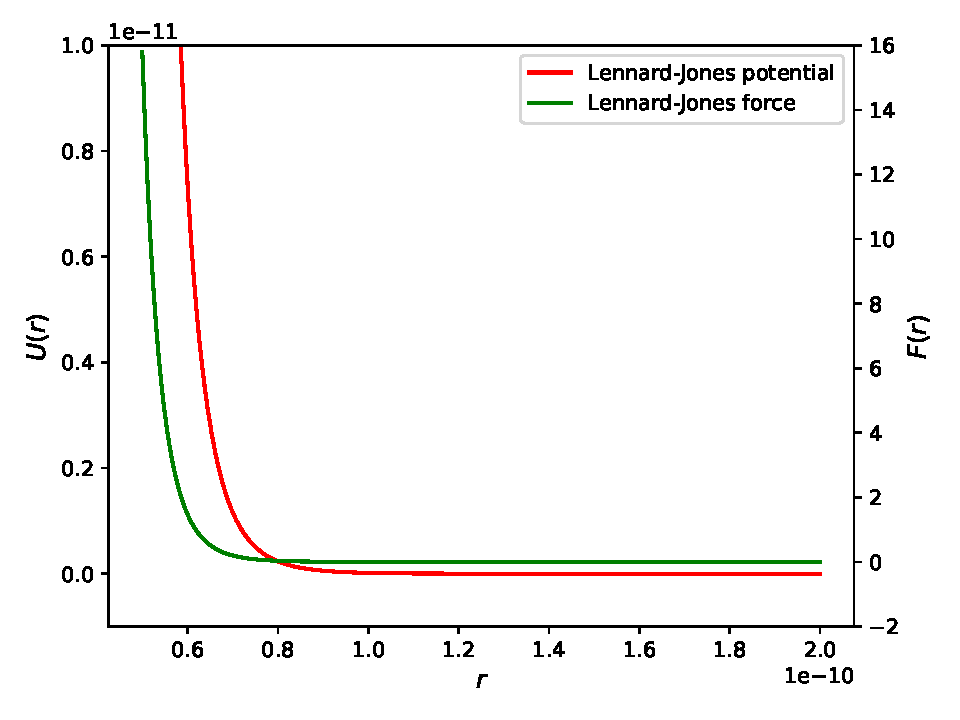
\includegraphics[width=0.5\linewidth]{lj_ar.pdf}
	\caption{Lennard--Jones potential and force for $\ce{Ar}$, as a function of
		distance between $2$ atoms, with
		$\sigma=3.405\times 10^{-10}\si{\meter}$,
		$\varepsilon = 1.654\times 10^{-21}\si{\joule}$.\cite{buffalomd}}
	\label{fig:ljar}
\end{figure}

Back to \texttt{FORCLJ} subroutine,
it considers 2 cases: particle $j$ and $i$ in the same cell and
in different cells, the first case is trivial, in the second case,
we need to add multiple times of primitive vectors and then calculate distance
$r_{ji}$, and the rest steps are the same as first case. In both cases, we do not
consider interaction out of the radius $r_{\text{cut}}$.
It appends \texttt{fo} and \texttt{fos} modified by \texttt{ELJ}
subroutine to the \texttt{f} and \texttt{fs}, respectively.


\subsubsection{\texttt{FORC} subroutine}

If \texttt{FORCLJ} is used for analytical computation, then this subroutine is
used as numerical methods.
We have talked about \texttt{RDPP} subroutine before, stating that it reads
$n (n+1)$ columns of potentials and forces, denoted as \texttt{vpp} and
\texttt{fpp}, respectively.
The potentials interpolated by quadratic functions, the forces are also
calculated similar process.


\subsubsection{\texttt{UPDG} subroutine}

This part is used to update several quantities of cell during calculations.

Here \texttt{avec} is $h$, \texttt{avecd} is $\dot{ h }$, thus $g = h\tran h$
and $\dot{g}  = \dot{ h }\tran h + h \dot{ h }\tran$, \texttt{gm1} is $g^{-1}$
and \texttt{gmgd} is $g^{-1} \dot{g}$. \texttt{sigma} is the reciprocal lattice
vectors $\sigma$.

It first reads a flag \texttt{itg} to see if $\sigma$ and $V$ need to be calculated,
if it is `yes', then do the following things:
Firstly calculates $\sigma$ by the components of $h$, and then calculate the
MD cell volume by
\begin{equation}
	V = \sigma \cdot h,
\end{equation}
and then calculate $g$, $\dot{ g }$, $g^{-1}$, $g^{-1}\dot{g}$, respectively.


\subsubsection{\texttt{SIGS} and \texttt{SIGP} subroutine}

\texttt{SIGS} subroutine is used to calculate lattice vectors accelerations
based on `new dynamics', i.e., according to $\eqref{eq:rpsdd}$ and
$\eqref{eq:wenzhdd}$; while \texttt{SIGP} is based on `strain dynamics',
i.e., $\eqref{eq:rpsdd}$ and $\eqref{eq:wenzhdd2}$. These $2$ routines
are called in \texttt{move} if \texttt{calc} is \texttt{sd} and \texttt{nd}, respectively.

In \texttt{SIGS} subroutine,
firstly calculates $f_0^{-1}$, by definition it is
\begin{equation}
	f_0^{-1} = \frac{ h_0 \tran h_0}{ V_0^2 },
\end{equation}
then set an argument \texttt{avint} to temporally store $\ddot{h}$,
and perform calculation $\ddot{h} = \ddot{h} f_0^{-1}$.

In \texttt{SIGP} subroutine,
firstly calculates $f^{-1}$, by definition we know it is
\begin{equation}
	f^{-1} = \frac{ h \tran h }{ V^2 },
\end{equation}
and $e = \dot{ h }\tran \dot{ h }$, as stated above, as well as
a $3\times 3 \times 3 \times 3$ tensor
\begin{equation}
	f ' = \frac{ \partial f }{ \partial h_{ij} } = (\sigma'_{ij})\tran \sigma
	+ \sigma \tran \sigma'_{ij},
\end{equation}
where $\sigma'$ is denoted as \texttt{sigmap} in code, another $3\times 3
	\times 3 \times 3$ tensor.
$\dot{f}_0 = \dot{ \sigma } \tran \sigma + \sigma \tran \dot{ \sigma }$ is
also calculated.
$f^{-1} = \sum_{k, l} e_{lk} f'_{ijkl}$, and $\sigma^{-1} = h \dot{ f }$.
Then final returns $\ddot{h}$. As stated above, $h = (1 + \epsilon) h_0$,
where $h_0 = \{ \bm{a}_0, \bm{b}_0, \bm{c}_0 \}$.


% !TEX root = ./report.tex

\subsection{Input file}

Now let's have a look at the input file.
A typical input file has structure like:
\begin{verbatim}
Test                              (title)
md                                (calc)
s       n                         (ic,iio)
10.00000                          (alatt)
1       1       1                 (nsc)
1.00000   0.00000   0.00000       (avec)
0.00000   1.00000   0.00000
0.00000   0.00000   1.00000
0.00100   0.00000                 (cmass, press)
1                                 (ntype)
4       Ar      36.00000          (natom,nameat,atmass)
0.00000   0.00000   0.00000       (rat)
0.50000   0.50000   0.00000
0.00000   0.50000   0.50000
0.50000   0.00000   0.50000
40                                (rcut)
6       6       6                 (ncell)
1000    100     10                (nstep,ntcheck,ntimes)
0.00000   0.00100   200.00000     (temp,ttol,dt)
\end{verbatim}

This input file investigates $4$ \ce{Ar} atoms in a FCC cell, the atom mass is assumed to be \SI{36.0}{\atomicmassunit},
see Fig. \ref{fig:fcc1} for the structure of this cell.
The \texttt{calc} specifies calculation type of this file, including \texttt{md},
\texttt{cd}, \texttt{nd}, \texttt{sd}, as we mentioned in the beginning of Sec. \ref{sec:mdc}.
\texttt{nsc} means the number of cells consist a supercell in each direction of a 3D space.
\texttt{cmass} is $W$ as mentioned, but it does not have functions for \texttt{md}.
\texttt{rcut} is the cut-off radius for this molecular dynamics, and the sphere defined by
\texttt{rcut} must be contained inside the stack of supercells, which is $7=2\times 3+1$ supercells in each direction. We usually choose numbers for \texttt{ncell}, to make
\texttt{alatt} times \texttt{ncell} greatly larger than \texttt{rcut}, for the supercells are
oscillating their volume in this molecular dynamics.
Here we have $4=4 \times 1^3$ atoms inside one supercell.
Make sure that \texttt{ntcheck} times \texttt{ntimes} is greater than
\texttt{nstep}.
And \texttt{dt} times \texttt{nstep} is the total simulation time in Rydberg unit, which is
\SI{4.8378e-17}{\second} per unit time.

\begin{figure}[H]
\begin{minipage}{0.48\textwidth}
	\centering
	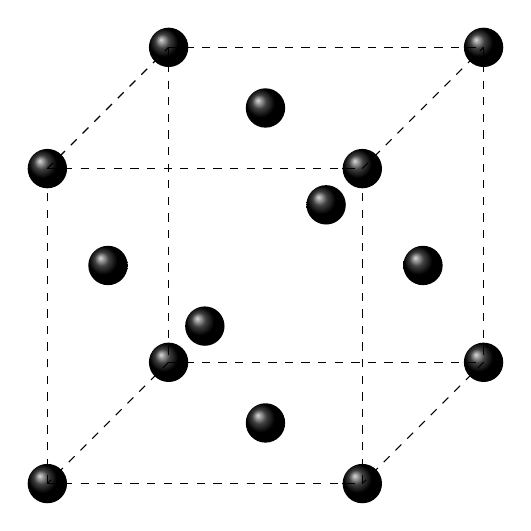
\begin{tikzpicture}
 %points on cube
 \coordinate (A) at (0,0,0);
 \coordinate (B) at (0,0,4);
 \coordinate (D) at (0,4,0);
 \coordinate (C) at (0,4,4);
 \coordinate (E) at (4,0,0);
 \coordinate (F) at (4,0,4);
 \coordinate (H) at (4,4,0);
 \coordinate (G) at (4,4,4);

 %center of faces
 \coordinate (I) at (0,2,2); %center of face ABCD
 \coordinate (J) at (4,2,2); %center of face EFGH
 \coordinate (K) at (2,4,2); %center of face DCGH
 \coordinate (L) at (2,0,2); %center of face ABFE
 \coordinate (M) at (2,2,4); %center of face CBGF
 \coordinate (N) at (2,2,0); %center of face DAEH

 %place non-atom cube corners
 \shade [ball color= black] (A) circle (0.25cm);
 \shade [ball color= black] (C) circle (0.25cm);
 \shade [ball color= black] (F) circle (0.25cm);
 \shade [ball color= black] (H) circle (0.25cm);
 \shade [ball color= black] (B) circle (0.25cm);
 \shade [ball color= black] (D) circle (0.25cm);
 \shade [ball color= black] (E) circle (0.25cm);
 \shade [ball color= black] (G) circle (0.25cm);

 %draw the center of each face
 \shade [ball color= black] (I) circle (0.25cm);
 \shade [ball color= black] (J) circle (0.25cm);
 \shade [ball color= black] (K) circle (0.25cm);
 \shade [ball color= black] (L) circle (0.25cm);
 \shade [ball color= black] (M) circle (0.25cm);
 \shade [ball color= black] (N) circle (0.25cm);

 %draw cube
 \draw [dashed] (A) -- (B);
 \draw [dashed] (B) -- (C);
 \draw [dashed] (C) -- (D);
 \draw [dashed] (D) -- (A);
 \draw [dashed] (E) -- (F);
 \draw [dashed] (F) -- (G);
 \draw [dashed] (G) -- (H);
 \draw [dashed] (H) -- (E);
 \draw [dashed] (A) -- (E);
 \draw [dashed] (B) -- (F);
 \draw [dashed] (C) -- (G);
 \draw [dashed] (D) -- (H);
\end{tikzpicture}

	\caption{A FCC conventional unit cell of \ce{Ar} for \texttt{inp1}.}
	\label{fig:fcc1}
\end{minipage}
\hfill
\begin {minipage}{0.48\textwidth}
\centering
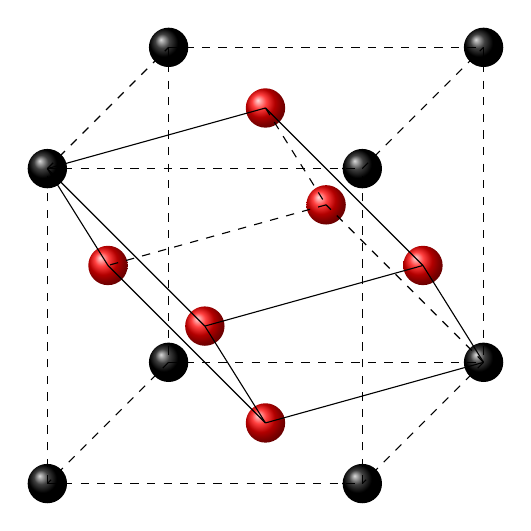
\begin{tikzpicture}
 %points on cube
 \coordinate (A) at (0,0,0);
 \coordinate (B) at (0,0,4);
 \coordinate (D) at (0,4,0);
 \coordinate (C) at (0,4,4);
 \coordinate (E) at (4,0,0);
 \coordinate (F) at (4,0,4);
 \coordinate (H) at (4,4,0);
 \coordinate (G) at (4,4,4);

 %center of faces
 \coordinate (I) at (0,2,2); %center of face ABCD
 \coordinate (J) at (4,2,2); %center of face EFGH
 \coordinate (K) at (2,4,2); %center of face DCGH
 \coordinate (L) at (2,0,2); %center of face ABFE
 \coordinate (M) at (2,2,4); %center of face CBGF
 \coordinate (N) at (2,2,0); %center of face DAEH

 %place non-atom cube corners
 \shade [ball color= black] (A) circle (0.25cm);
 \shade [ball color= black] (C) circle (0.25cm);
 \shade [ball color= black] (F) circle (0.25cm);
 \shade [ball color= black] (H) circle (0.25cm);
 \shade [ball color= black] (B) circle (0.25cm);
 \shade [ball color= black] (D) circle (0.25cm);
 \shade [ball color= black] (E) circle (0.25cm);
 \shade [ball color= black] (G) circle (0.25cm);

 %draw the center of each face
 \shade [ball color= red] (I) circle (0.25cm);
 \shade [ball color= red] (J) circle (0.25cm);
 \shade [ball color= red] (K) circle (0.25cm);
 \shade [ball color= red] (L) circle (0.25cm);
 \shade [ball color= red] (M) circle (0.25cm);
 \shade [ball color= red] (N) circle (0.25cm);

 %draw cube
 \draw [dashed] (A) -- (B);
 \draw [dashed] (B) -- (C);
 \draw [dashed] (C) -- (D);
 \draw [dashed] (D) -- (A);
 \draw [dashed] (E) -- (F);
 \draw [dashed] (F) -- (G);
 \draw [dashed] (G) -- (H);
 \draw [dashed] (H) -- (E);
 \draw [dashed] (A) -- (E);
 \draw [dashed] (B) -- (F);
 \draw [dashed] (C) -- (G);
 \draw [dashed] (D) -- (H);
 
 %draw unit cell
 \draw (E) -- (L);
 \draw (E) -- (J);
 \draw [dashed] (E) -- (N);
 \draw (J) -- (M);
 \draw (L) -- (M);
 \draw (J) -- (K);
 \draw [dashed] (K) -- (N);
 \draw (K) -- (C);
 \draw (M) -- (C);
 \draw (L) -- (I);
 \draw [dashed] (N) -- (I);
 \draw (C) -- (I);
\end{tikzpicture}

\caption{A FCC primitive unit cell of \ce{Ar} for \texttt{inp3}, with
	vertices of the cell filled in red.}
\label{fig:fcc3}
\end{minipage}
\end{figure}

Now we are going to play with Wentzcovitch's molecular dynamics, to see what the
actual ``dynamics'' it is. Suppose we have such a file as \texttt{inp1}:
\begin{verbatim}
Test                              (title)
nd                                (calc)
s       n                         (ic,iio)
11.00000                          (alatt)
1       1       1                 (nsc)
1.00000   0.00000   0.00000       (avec)
0.00000   1.00000   0.00000
0.00000   0.00000   1.00000
0.00100   0.00000                 (cmass, press)
1                                 (ntype)
4       Ar      36.00000          (natom,nameat,atmass)
0.00000   0.00000   0.00000       (rat)
0.50000   0.50000   0.00000
0.00000   0.50000   0.50000
0.50000   0.00000   0.50000
40                                (rcut)
6       6       6                 (ncell)
2000    100     10                (nstep,ntcheck,ntimes)
0.00000   0.00100   75.00000      (temp,ttol,dt)
\end{verbatim}
We will use this file as an example for comparison.
The \texttt{press} is external pressure $P$, but in unit of \si{\mega\bar}.

Here we are going to use $h = 75$ Rydberg unit and $2000$ time steps. This is because, different \texttt{dt} could result in different decaying rates.
We run this file with $4$ different \texttt{dt}, $150$, $200$, $300$ and $400$
Rydberg unit respectively.
But we simulate both $600000$ Rydberg time unit. From Fig. \ref{fig:inp1:mini:subfig:b} we can see a noticeable
decreasing in total energy, but for Fig. \ref{fig:inp1:mini:subfig:a} this is less distinguishable. For Fig. \ref{fig:inp1:mini:subfig:c} and Fig. \ref{fig:inp1:mini:subfig:d}
this is even worse, the total energy decays even faster. This can be understood since in
Beeman's algorithm we assume the length of each time step $h$ is a small quantity,
for we are using Taylor expansion implicitly. So when $h$ is too large, numerical errors
could be apparent.

\begin{figure}[h]
	\centering
	\subfigure[$4000$ time steps, with each time step to be $150$ Rydberg unit.]{
		\label{fig:inp1:mini:subfig:a}   %% label for second subfigure 
		\begin{minipage}[b]{0.48\textwidth}
			\centering
			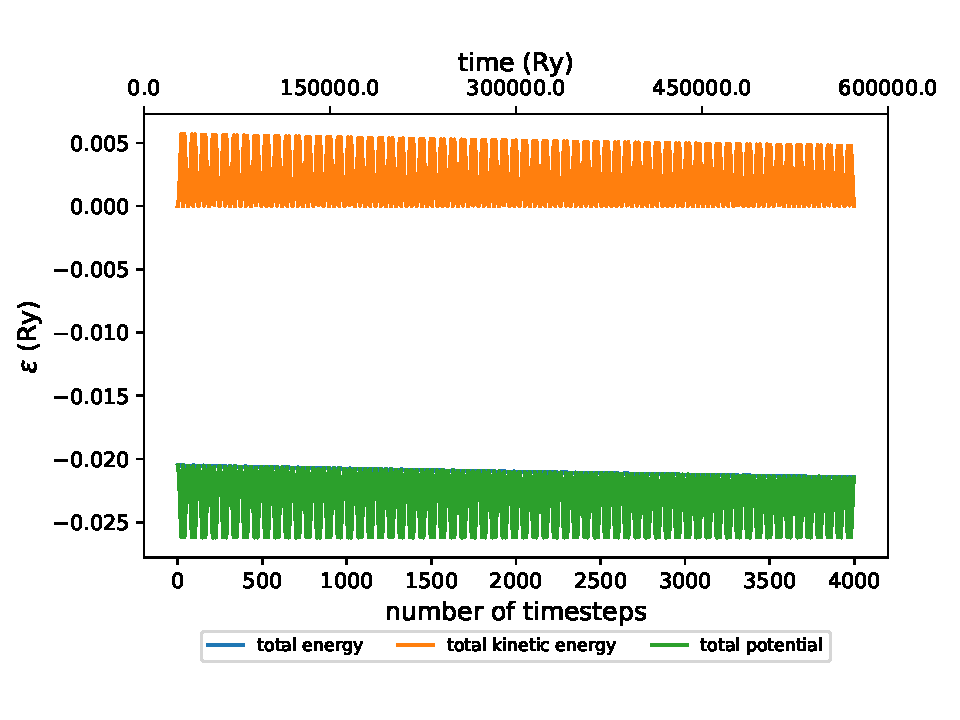
\includegraphics[width=\linewidth]{4000_150_100_4}
		\end{minipage}}
	\hfill
	\subfigure[$3000$ time steps, with each time step to be $200$ Rydberg unit.]{
		\label{fig:inp1:mini:subfig:b}   %% label for first subfigure 
		\begin{minipage}[b]{0.48\textwidth}
			\centering
			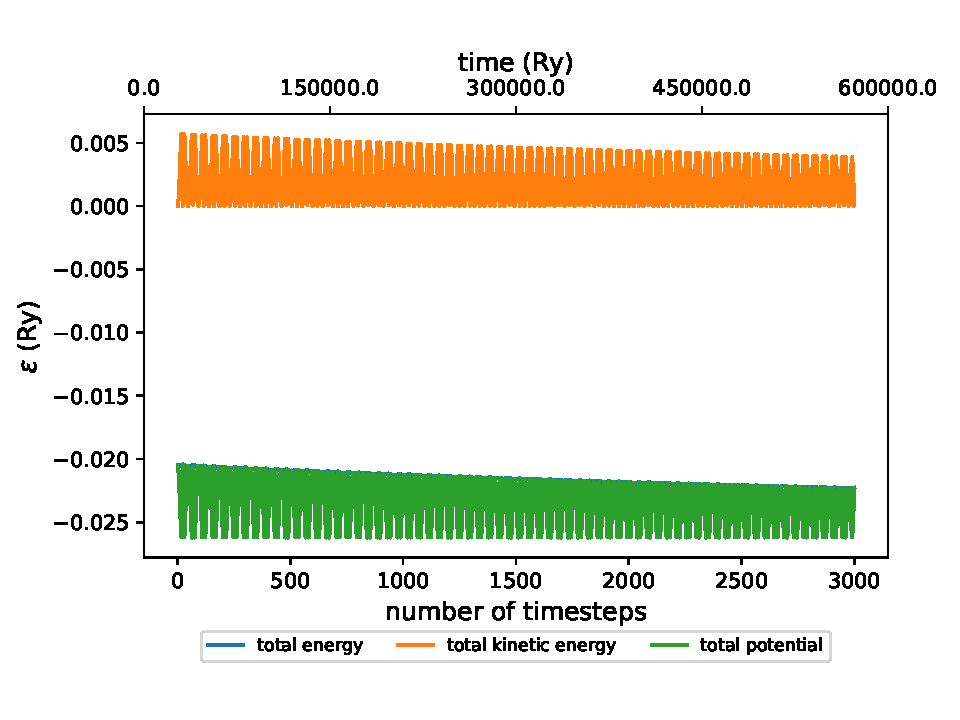
\includegraphics[width=\linewidth]{3000_200_100_9}
		\end{minipage}}
	\subfigure[$2000$ time steps, with each time step to be $300$ Rydberg unit.]{
		\label{fig:inp1:mini:subfig:c}   %% label for third subfigure 
		\begin{minipage}[b]{0.48\textwidth}
			\centering
			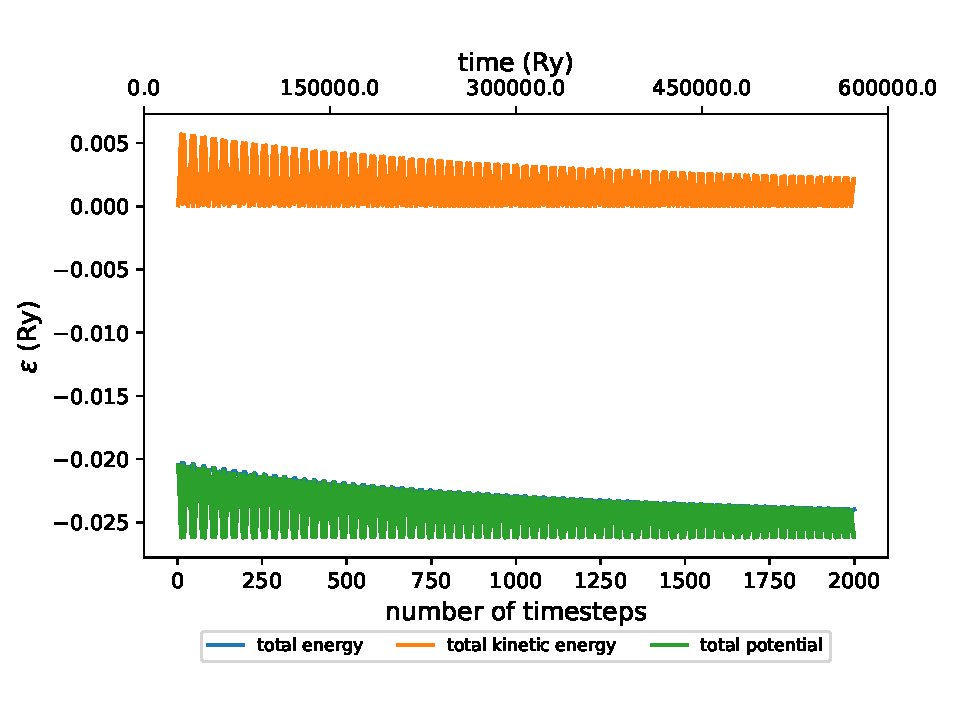
\includegraphics[width=\linewidth]{2000_300_100_0}
		\end{minipage}}
	\hfill
	\subfigure[$1500$ time steps, with each time step to be $400$ Rydberg unit.]{
		\label{fig:inp1:mini:subfig:d}   %% label for fourth subfigure 
		\begin{minipage}[b]{0.48\textwidth}
			\centering
			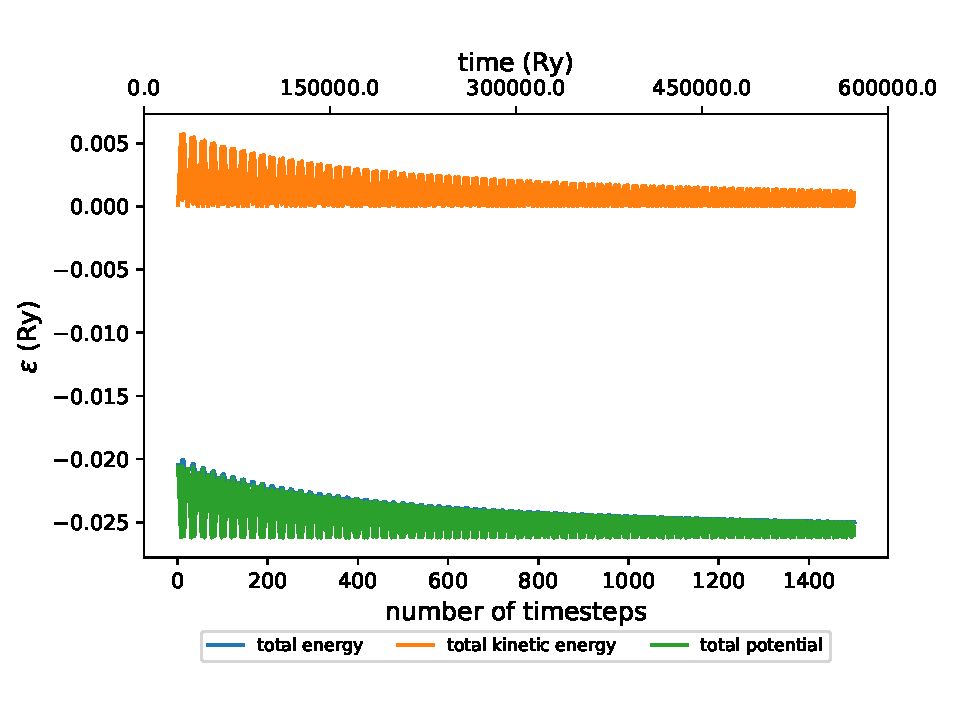
\includegraphics[width=\linewidth]{1500_400_100_2}
		\end{minipage}}
	\caption{Wentzcovitch MD for FCC \ce{Ar} at \SI{0}{\kelvin} with $4$ different \texttt{dt} but the same total simulation time.}
	\label{fig:inp1}   %% label for entire figure 
\end{figure}

So for easier observation $h = 75$ Rydberg unit and $2000$ time steps are good choices,
see Fig. \ref{fig:inp1run} for references.

\begin{figure}[h]
	\subfigure[Energies of the cell and atoms versus time.]{
		\label{fig:inp1run:mini:subfig:a}   %% label for first subfigure 
		\begin{minipage}[b]{0.48\textwidth}
			\centering
			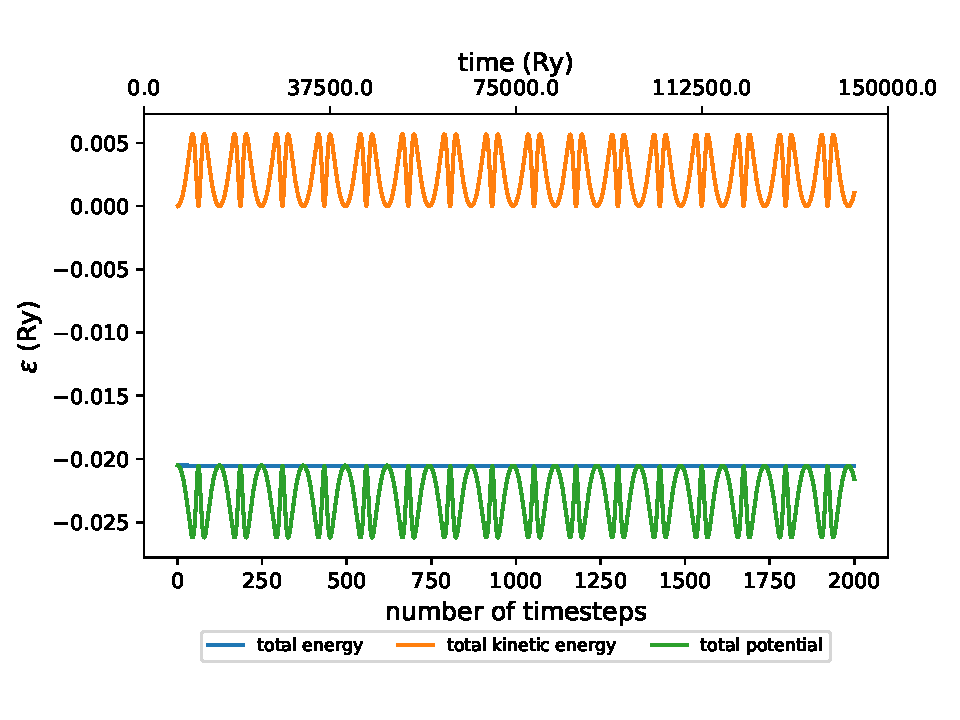
\includegraphics[width=\linewidth]{2000_75_100_8}
		\end{minipage}}
	\hfill
	\subfigure[Cell vectors oscillation versus time, $a=b=c$ for this is a cubic crystal.]{
		\label{fig:inp1run:mini:subfig:b}   %% label for second subfigure 
		\begin{minipage}[b]{0.48\textwidth}
			\centering
			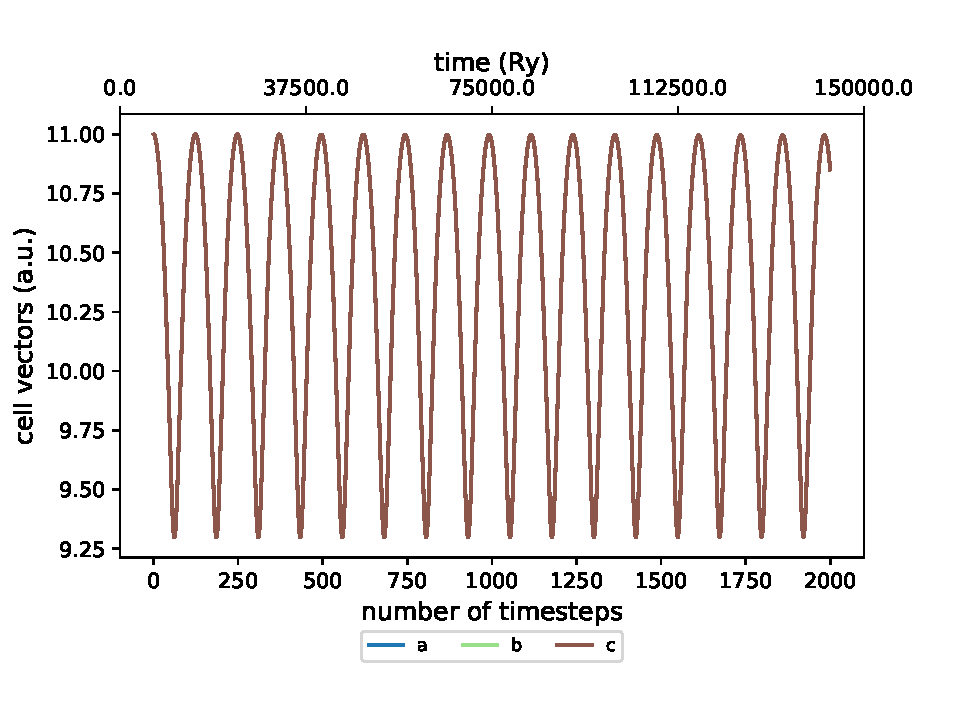
\includegraphics[width=\linewidth]{2000_75_100_2_avec}
		\end{minipage}}
	\caption{Wentzcovitch MD for FCC \ce{Ar} at \SI{0}{\kelvin}, with \texttt{dt}$=75$,
		\texttt{nstep}$=2000$.}
	\label{fig:inp1run}   %% label for entire figure 
\end{figure}

From Fig. \ref{fig:inp1run:mini:subfig:b} we can approximate assume that the stable
lattice parameter is around \SI{9.9}{\bohr}, where vibration happens back and forth.
But the code also provide a \texttt{nm} method by adding a damping to let us compute energy-minimized structure quickly. So we keep the fictitious mass fixed,
and then run the structure minimization algorithm. The stabilized structure also has a
lattice parameter around \SI{9.9}{\bohr}, which strengthen the credibility of our MD result,
see Fig. \ref{fig:inp5} for references.

\begin{figure}[h]
  \subfigure[Energies for structure minimization versus time.]{
    \label{fig:inp5:mini:subfig:a}   %% label for first subfigure 
    \begin{minipage}[b]{0.48\textwidth}
      \centering
      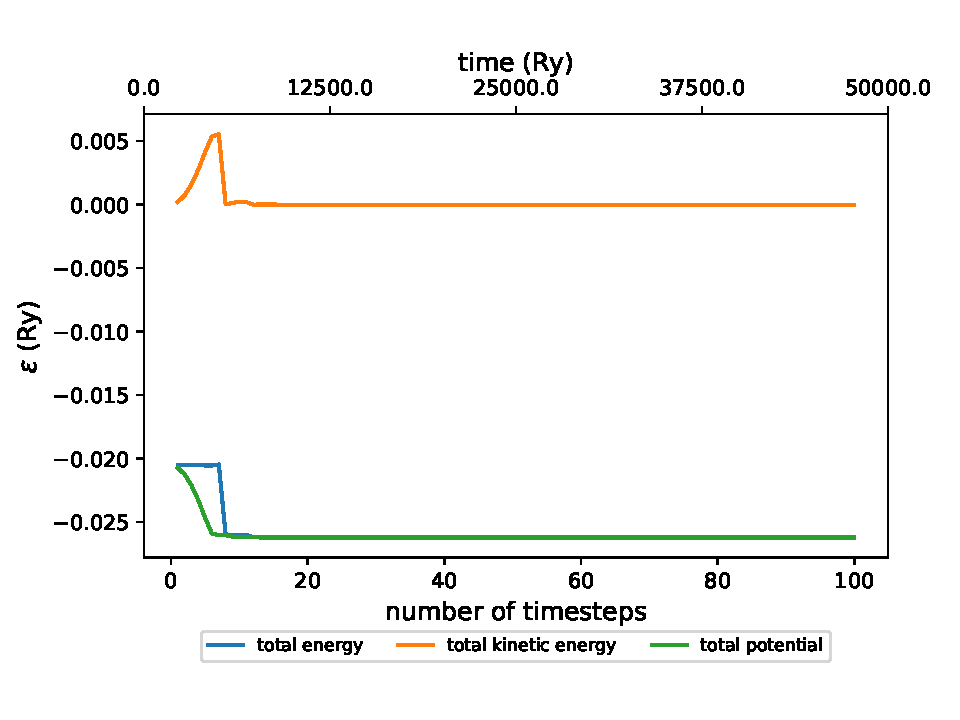
\includegraphics[width=\linewidth]{100_500_2010_9}
  \end{minipage}}
  \hfill
  \subfigure[Lattice parameters for structure minimization versus time, the final result is around \SI{9.9}{\bohr}.]{
    \label{fig:inp5:mini:subfig:b}   %% label for second subfigure 
    \begin{minipage}[b]{0.48\textwidth}
      \centering 
      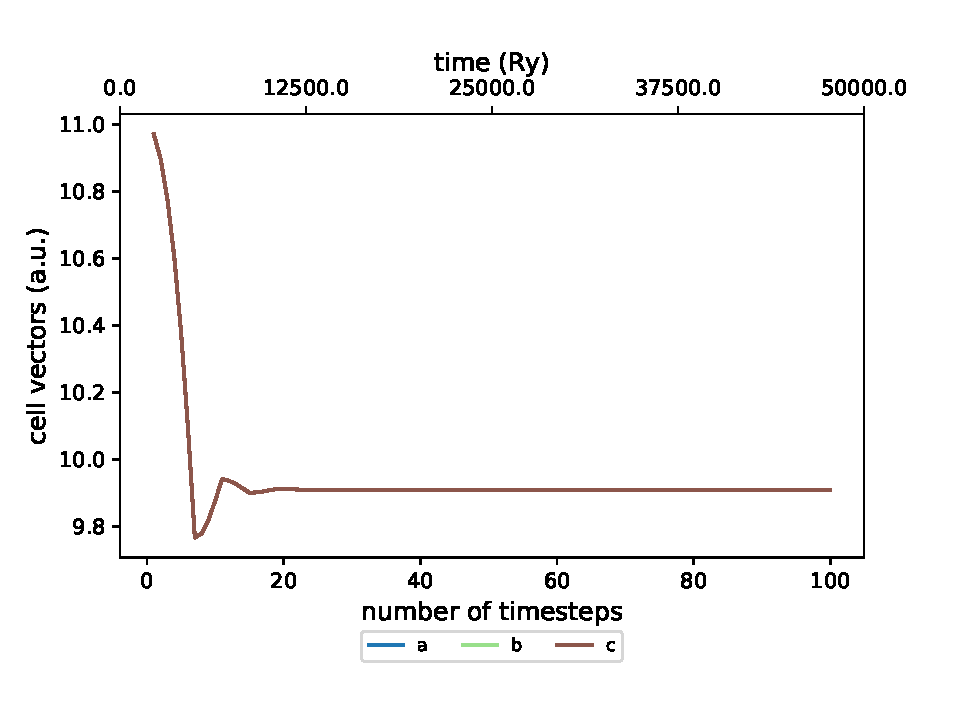
\includegraphics[width=\linewidth]{100_500_2010_3_avec} 
  \end{minipage}}
  \caption{Wentzcovitch's structure minimization algorithm for FCC \ce{Ar}.}
  \label{fig:inp5}   %% label for entire figure 
\end{figure}


First we run the code using Andersen's molecular dynamics, to find the oscillation frequency of atoms. This is done at \SI{0}{\kelvin}, so we have to shift the atoms a little from their equilibrium
positions, or else we will not observe an oscillation frequency, like in Fig. \ref{fig:andersen0:mini:subfig:a}.
For example, in Fig. \ref{fig:andersen0:mini:subfig:b} we can approximately assume that
one period of oscillation is $110$ time steps. We will use this quantity later.
\begin{figure}[h]
	\centering
	\subfigure[Every atom sits in exactly their equilibrium coordinates.]{
		\label{fig:andersen0:mini:subfig:a}   %% label for first subfigure 
		\begin{minipage}[b]{0.48\textwidth}
			\centering
			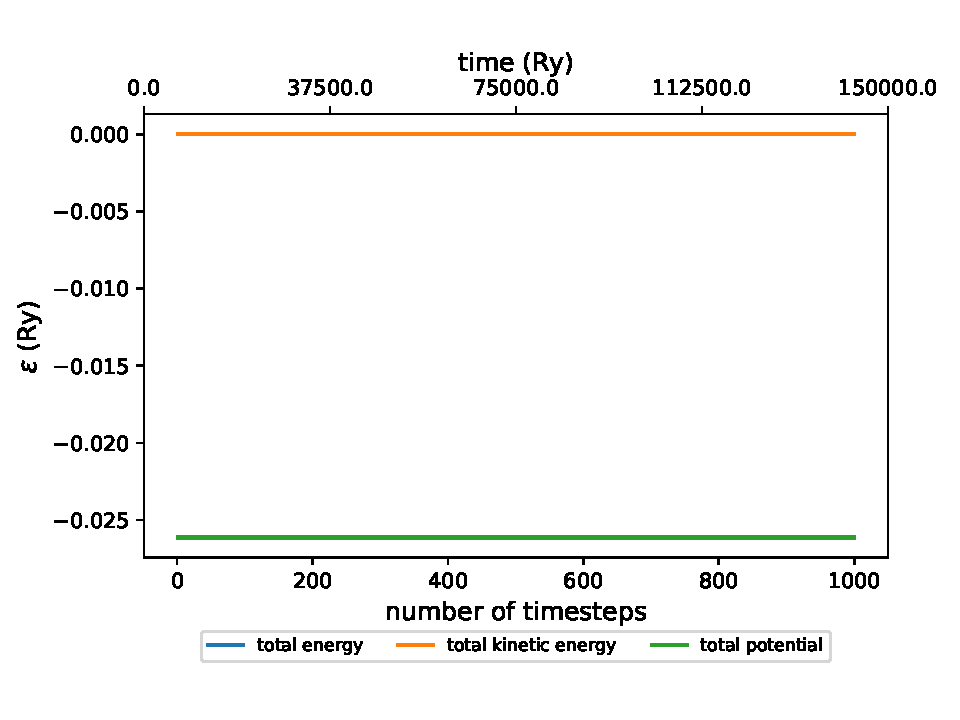
\includegraphics[width=\linewidth]{1000_150_1100_2.pdf}
		\end{minipage}}
	\hfill
	\subfigure[One of the atom shifts a little upon its equilibrium coordinate.]{
		\label{fig:andersen0:mini:subfig:b}   %% label for second subfigure 
		\begin{minipage}[b]{0.48\textwidth}
			\centering
			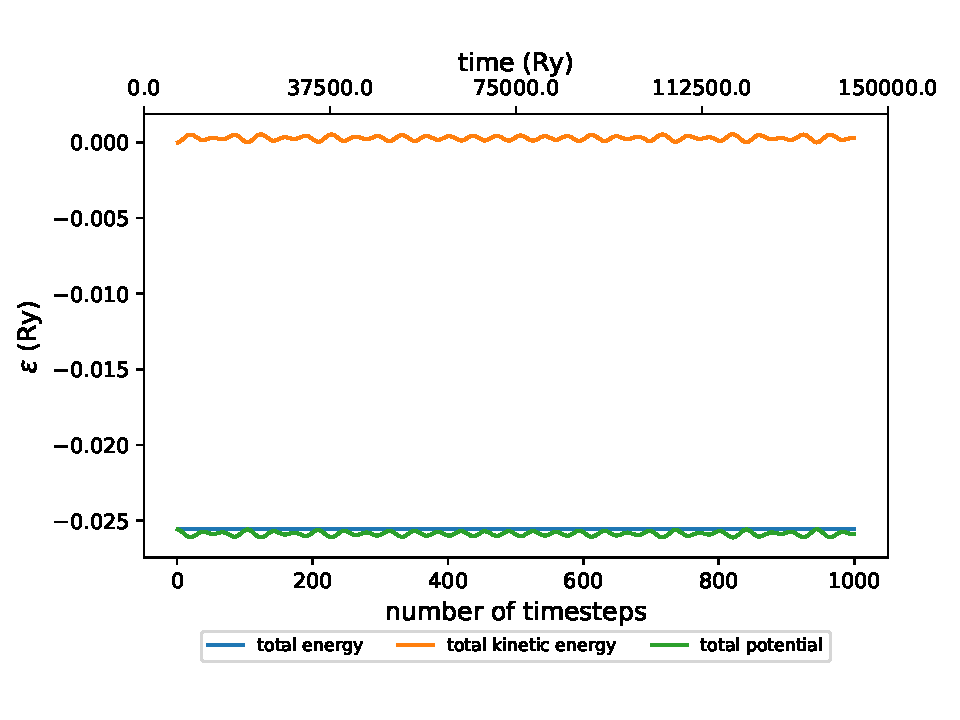
\includegraphics[width=\linewidth]{1000_150_1100-3.pdf}
		\end{minipage}}
	\caption{A conventional FCC cell of \ce{Ar} at \SI{0}{\kelvin}}
	\label{fig:andersen0}   %% label for entire figure 
\end{figure}


%If we keep all other simulation parameters the same, but change
%the size of time steps to $100$ in \texttt{inp2} (\texttt{inp1} is $200$) in Rydberg-like units,
%i.e., decrease step size by a half, the results will be shown in Fig. \ref{fig:input2}.
%There is not much differences from the first results. But looking in detail,
%we can see that the amplitude of atomic potential in Fig. \ref{fig:input2:a} is not decaying
%and the amplitude of lattice kinetic energy in Fig. \ref{fig:input2:l} is also not decaying
%comparing to the corresponding figures Fig. \ref{fig:input1:a} and Fig. \ref{fig:input1:l},
%respectively. And also, the amplitude of lattice parameter is not decaying in
%Fig. \ref{fig:input2:avec} rather than in \ref{fig:input1:avec}. We should also be aware of
%that the oscillation frequency of energies, including kinetic and potential, do not change
%as the time step is decreased to $\frac{ 1 }{ 2 }$, we will discuss later on this phenomenon.
%\begin{figure}[H]
%  \begin{minipage}[t]{0.45\textwidth}
%    \includegraphics[width=\linewidth]{input2/avec_abc}
%    \subcaption{Lattice parameters of \texttt{inp2}.}
%    \label{fig:input2:avec}
%  \end{minipage}
%  \hfil
%  \begin{minipage}[t]{0.45\textwidth}
%    \includegraphics[width=\linewidth]{input2/t}
%    \subcaption{Total energy of \texttt{inp2}.}
%    \label{fig:input2:t}
%  \end{minipage}
%  \hfil
%  \vfill
%  %\vspace*{0.5cm} % (or whatever vertical separation you prefer)
%  \begin{minipage}[t]{0.45\textwidth}
%    \includegraphics[width=\linewidth]{input2/a}
%    \subcaption{Atomic contribution to total energy of \texttt{inp2}.}
%    \label{fig:input2:a}
%  \end{minipage}
%  \hfil
%  \begin{minipage}[t]{0.45\textwidth}
%    \includegraphics[width=\linewidth]{input2/l}
%    \subcaption{Lattice contribution to total energy of \texttt{inp2}.}
%    \label{fig:input2:l}
%  \end{minipage}
%  \caption{Simulation results for \texttt{inp2}.}
%  \label{fig:input2}
%\end{figure}

For \texttt{inp3}, now we shrink the unit cell size to $\frac{ 1 }{ 4 }$ of the
\texttt{inp1}, i.e., there is only $1$ \ce{Ar} atom in the cell. 
Also, the time step is $100$, the same as \texttt{inp2}.
See Fig. \ref{fig:fcc3} for reference.
Now let's see what will happen to the simulation result. 

However, this time, the oscillation frequency of energies and lattice parameters
both increase by a factor of $2$, this is not astonishing because from
\eqref{eq:hdd} we know that
\begin{equation}
	\omega \propto \sqrt{
		\frac{ B }{ W V }
	},
\end{equation}
where $B$ is the bulk modulus.
Here we again see the decaying phenomenon,
comparing to simulation of \texttt{inp1}, we see that the oscillation amplitude of
both
%\begin{figure}[H]
%  \begin{minipage}[t]{0.45\textwidth}
%    \includegraphics[width=\linewidth]{input3/avec_abc}
%    \subcaption{}
%    \label{fig:input3:avec_abc}
%  \end{minipage}
%  \hfil
%  \begin{minipage}[t]{0.45\textwidth}
%    \includegraphics[width=\linewidth]{input3/t}
%    \subcaption{}
%    \label{fig:input3:t}
%  \end{minipage}
%  \hfil
%  \vfill
%  %\vspace*{0.5cm} % (or whatever vertical separation you prefer)
%  \begin{minipage}[t]{0.45\textwidth}
%    \includegraphics[width=\linewidth]{input3/a}
%    \subcaption{}
%    \label{fig:input3:a}
%  \end{minipage}
%  \hfil
%  \begin{minipage}[t]{0.45\textwidth}
%    \includegraphics[width=\linewidth]{input3/l}
%    \subcaption{}
%    \label{fig:input3:l}
%  \end{minipage}
%  \caption{\texttt{inp3}.}
%  \label{fig:input3}
%\end{figure}


\bibliography{thebib}
\nocite{dufty1986molecular}
\end{document}
